\chapter{Palabras acumuladas}
% Intro {{{

La búsqueda para cuantificar la influencia, ha llevado a contabilizar las
palabras que son nuevas en los distintos receptores, para después encontrar relaciones históricas que sustenten su aparición.  El tratamiento anterior sólo se ha hecho en los años del conjunto de búsqueda, pero  el conjunto base  también tiene información sobre las migraciones, además abarca más años (159 comprendidos entre 1740 y 1899), por lo que su contenido es más amplio. 

\jmnote{el siguiente parrafo lo rescribi, las 3 siguientes notas que me dejaste eran referentes al pparafo antes de rescribirlo.}

%$\rightarrow$ 

%\fxwarning{Rescribi  de forma mas compacta casi todo el contenido de esta pagina, tratando de ser mas claro respecto a las notas que me dejaste, deje la flecha para indicar lo que habia escrito no borrar donde dejaste notas. }

%Para no repetir el proceso de contabilizar a los préstamos nuevos,  se propone pensar que en el primer año del conjunto de búsqueda (1900), el idioma receptor ya contenia  cierta cantidad de palabras que provenian de otros origenes; de tal manera que  ya forman parte de él, es decir estos préstamos ``conviven'' con las palabras propias de el receptor y son empleadas indistintamente



%Así el conjunto base proporcionará un sostén de aquellas palabras que han permeado en un idioma
%y son utilizadas en los años del conjunto de búsqueda,  cabe decir que este
%sostén crecerá conforme se localicen nuevas palabras\cpnote{acá tampoco entiendo}. 

%Es necesario hacer una nueva definición para estos préstamos, dados un idioma  origen  \textit{A} y la lista para un año  de las palabras más comunes en el receptor \textit{B}, se definen como: 

%\begin{description}
	%\item[préstamos acumulados:] Son las palabras con origen \textit{A} que ya habían aparecido en alguna lista de \textit{B}, y para ese año lo volvieron a hacer.  \cpnote{Es decir que volvieron a aparecer, o que siguen estando? no me queda claro. En la frase despues, lo aclaras, pero siento que la definicion está deficiente. Igual porfa no quites la siguiente frase.}
%\end{description}
%$\rightarrow$



Para trabajar con la información del conjunto base, se buscan los préstamos nuevos de \textit{A} en \textit{B}, durante los años de este conjunto (1740-1899).  En este punto, conviene definir como \textbf{préstamos acumulados} a aquellas palabras  con origen \textit{A} que ya habían aparecido en \textit{B}, y para un determinado año lo vuelven a hacer. 

La diferencia entre los nuevos y los acumulados, es que un préstamo será nuevo sólo en el año de aparición, posteriormente se convertirá en acumulado.  Ya que en cada año hay más palabras acumuladas que palabras nuevas, al trabajar con acumulados se esta evitando tener años sin palabras migrantes, aspecto común en los préstamos nuevos. 


\cpnote{A que te refieres con orígenes?}

\cpnote{No entiendo lo que quieres decir en esta frase.  Sugiero que la redactes mejor o me la expliques en persona.}

\cpnote{No entiendo porque cambias el formato. Sugiero seguir con el parrafo como va. De hecho veo que en el capitulo 3, al principio tienes un formato similar. Cambia ambos e integralos en el texto. En la seccion 2.2 me gusta como tienes esas primeras 4 definiciones. Las primeras dos, integradas en una frase, y las siguientes dos, como parte de una frase dentro de items. }





Además de la cantidad, la frecuencia de los préstamos acumulados es relevante para obtener una cantidad medible  con la cual interpreta la influencia. Para lograr tal cantidad, se realizaron los siguientes pasos.

\cpnote{Que quieres decir con esa ultima frase? Que comportamiento? No se que podemos decir con los datos que tenemos}.  
\jmnote{Para aclarar la frase que esta comentada,  es mejor definir antes las cantidades que quiero medir y aclarar que puedo interpretsar de ellas.}


\cpnote{Oye, no me queda claro que estas usando el doble punto de manera
	correcta. Puedes porfa verificar en un manual de ortografía y gramática que lo estas haciendo bien?}
\jmnote{No lo estaba haciendo bien,  para enumerar o detallar un proceso no se usan los dos puntos,    lo comprobe en una pagina de la UAM, corrijo en donde haya hecho lo mismo http://www.uamenlinea.uam.mx/materiales/lengua/puntuacion/html/puntos.htm 
}


\begin{enumerate}
	\label{proceso_uso}
	
	\item  Dada la lista de las cinco mil palabras mas usadas de \textit{B} en el año $t$, se obtiene la \textbf{frecuencia total} $\underset{\text{\tiny B}}{F}(t)$ al sumar las frecuencias $f(k)$ de todas las palabras en la lista, donde $k$ determina el rango  de cada palabra.
	
	\begin{equation}
	\label{ec.ftot}
	%F^{y}_{\text{B}} = \sum_{k=1}^{5000} f(k)
	\underset{\text{\tiny B}}{F}(t) = \sum_{k=1}^{5000} f(k)
	\end{equation}
	
	\cpnote{el texto en una ecuaccion se pone de otra manera. Además, no
		tienes necesitad de ponerlo ahi, mejor en lo que sigue. Ademas, tu
		notacion esta chafa. Si tenemos $f_5$ es a tiempo 5 o para el rango 5?
		Dale una iterada a todo este capitulo. Veo que 
		no esta tan pulida como otros capitulos.} 
	\jmnote{Listo, corregida y el texto lo puse dentro del punto y ya no en la ecuacion}
	
	
	\item Si se distinguen los préstamos acumulados con origen \textit{A}  que tienen rango $j$,  se procede a sumar la frecuencia $f(j)$ de estas palabras.  Esta cantidad será la  \textbf{frecuencia de préstamo} $\underset{ \text{\tiny A} \to  \text{\tiny B} }{P}(t)$   de \textit{A} en \textit{B} para el año $t$.
	
	\begin{equation}
	\label{ec.fpres}
	%P^{y}_{\text{A} \to \text{B}} = \sum_{j} f(j)
	\underset{ \text{\tiny A} \to  \text{\tiny B} }{P}(t) = \sum_{j} f(j)
	\end{equation}
	
	
	\item  Al dividir la frecuencia de préstamo entre la frecuencia total, se obtiene el uso \textbf{uso} $\underset{ \text{\tiny A} \to  \text{\tiny B} }{U}(t)$  de \textit{A} en \textit{B}.  
	
	\begin{equation}
	\label{ec.fuso}
	\underset{ \text{\tiny A} \to  \text{\tiny B} }{U}(t) = \frac{	\underset{ \text{\tiny A} \to  \text{\tiny B} }{P}(t)}{\underset{\text{\tiny B}}{F}(t) } * 100
	\end{equation}
	
	\jmnote{deje los subindices para saber que opinabas,  a mi gusto se ve saturado y  creo que se sobrentiende que al tener el subindice bajo  la U, que  P y F también lo  tienen. }
	
	Este  nuevo valor será el que cuantifique la influencia, sin embargo al ser una cantidad pequeña, se tomará como un porcentaje al multiplicar el cociente por cien, obteniendo cifras manejables. 
	
	%\item Se empleó la ecuación \ref{ec.fuso} en todos los años del conjunto de búsqueda, obteniendo 109 valores.
	
	%\item El proceso se repitió para todas las combinaciones de orígenes y receptores.
	
\end{enumerate}

El objetivo de trabajar con los acumulados, es ver el comportamiento de las palabras que ya han migrado a un receptor, observando si hay periodos donde su empleó (a través del uso) se vea alterado. 

Para aclarar la última idea, en una lista del receptor \textit{B}, se encuentran  préstamos acumulados con diferentes orígenes \textit{A}, \textit{C} o \textit{D}, cada uno tiene un valor propio de uso. Como el uso depende del tiempo, a lo largo de los años, se pueden estimar las épocas donde algún origen tiene un mayor uso dentro de \textit{B},  en consecuencia una mayor influencia. 

Al igual que en los préstamos nuevos,  se agruparon los préstamos acumulados por cada pareja de origen y receptor,  y dentro de ella, un segundo listado por cada año de búsqueda.  Se proporciona en \cite{prestamos_acumulados} las agrupaciones realizadas, mientras que en \ref{palabras.acumuladas.apendice} se especifica la forma de leerlas e interpretarlas. 



\section {El uso entre idiomas} 

Para la influencia entre idiomas, se obtuvo el uso de un idioma en otro entre los años de 1740 y 2009. Para ser acordes al periodo donde se buscaron los préstamos nuevos, solo se discutirán los resultados obtenidos en los años del conjunto de búsqueda (1900-2009).


Por cada idioma se presentan dos graficas, la primera al fijar un origen para observar el uso que tiene en los demás; la segunda es el caso contrario,  al graficar el uso de los demás en el.  Una tercera grafica es posible, al representar unicamente el uso entre dos idiomas, estas graficas se agregaran en la sección \ref{palabras.acumuladas.apendice} del Apéndice A.

Para complementar los resultados del capitulo anterior, se expondrán las palabras que intervienen en las épocas donde el uso se vea alterado, estas palabras son las que año con año cambian su frecuencia, tras ascender o descender en posiciones de rango. 

Adicionalmente, la tabla \ref{tab.cantidad_acumulados} muestra la cantidad promedio de préstamos acumulados, encontrados en el conjunto de búsqueda. La idea  entre la tabla y del uso, es notar que el idioma que más palabras aporta a un receptor no es siempre el de mayor uso.  El uso es mayor si los préstamos tienen rangos mas bajos(frecuencias altas), sin importar cuantos sean. 


\begin{table}
	\centering
	\begin{tabular}{lcccccc}
		\multicolumn{7}{c}{R E C E P T O R}                                                                                                                                             \\
		\multirow{6}{*}{\begin{tabular}[c]{@{}l@{}}O\\ R\\ \,I\\ G\\ E\\ N\end{tabular}} &             & \textbf{inglés} & \textbf{francés} & \textbf{alemán} & \textbf{italiano} & \textbf{español} \\
		& \textbf{inglés} & -           & 324.43      & 164.33      & 77.5        & 73.61       \\
		& \textbf{francés} & 297.36      & -           & 94.06       & 118.55      & 66.31       \\
		& \textbf{alemán} & 63.87       & 48.06       & -           & 34.92       & 16.61       \\
		& \textbf{italiano} & 77.82       & 100.62      & 47.9        & -           & 219.45      \\
		& \textbf{español} & 118.43      & 84.22       & 29.85       & 311.97      & -          
	\end{tabular}
	\caption{Promedio de préstamos acumulados entre idiomas. Se aprecian dos relaciones reciprocas entre el inglés con el francés y el español con el italiano, donde no importa cual actué como receptor, el otro idioma es el origen del que provienen la mayor cantidad de palabras.}
	\label{tab.cantidad_acumulados}
\end{table}



\subsection{Inglés} % {{{

\jmnote{Personalmente, me agrada la presentación de una grafica y su descripción, no me agrada como acomoda latex la figura y el texto, supongo que estos detalles se arreglaran al final.}

\begin{figure}%[h!]
	\centering
	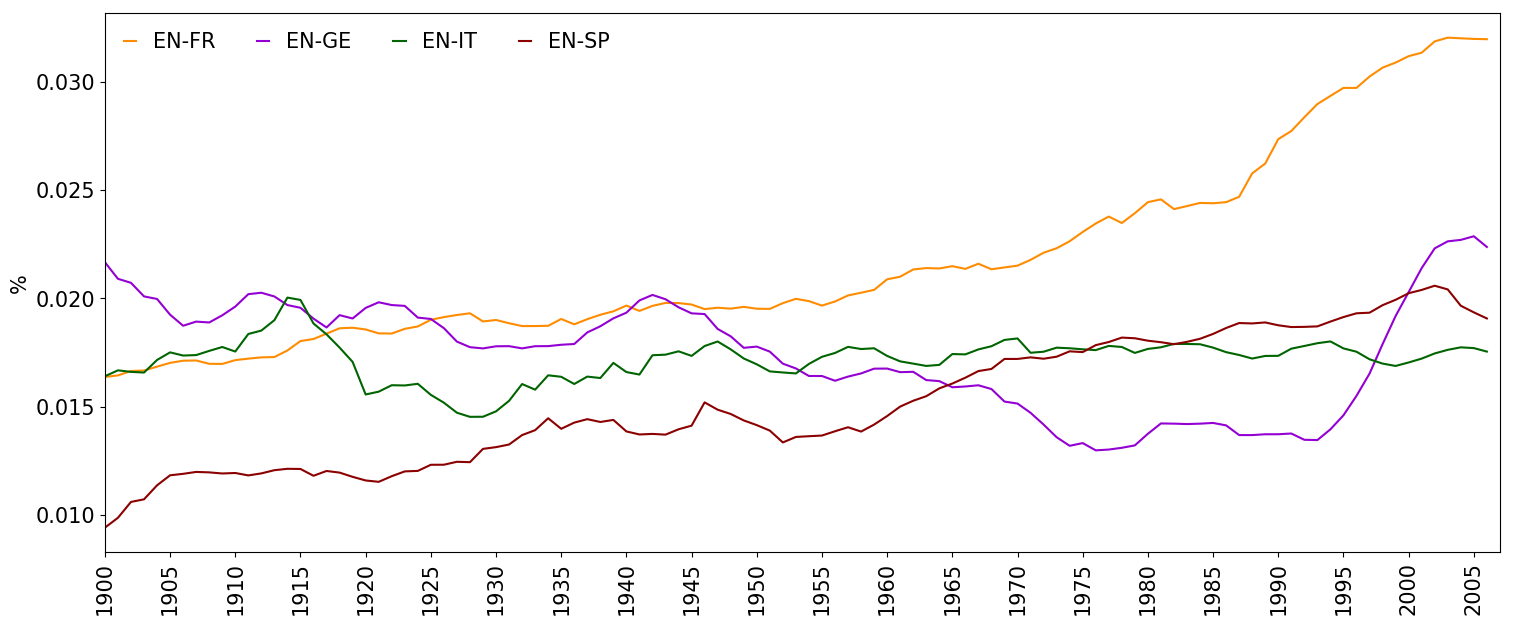
\includegraphics[scale=.36]{PF1_S2_EN.png}
	\label{fig.ST_a_EN}
	\caption{El inglés en los demás idiomas. Todos los idiomas han empleado más al inglés en la segunda mitad del siglo XX, destacando el mayor uso por parte del francés.}
\end{figure} 



El uso del ingles en el francés, el italiano y el español , aumentó constantemente a partir de 1945, tras finalizar la segunda guerra mundial, en cambio en el alemán, su uso decayó después de 1945, no obstante a partir de 1990 ha sido el idioma con el mayor aumento.

El significado común de los préstamos acumulados  en los cuatro receptores,  son términos referentes a la industria  y a la economía, entre ellos \textit{capital}, \textit{dollar}, \textit{invesment}, \textit{relations}, \textit{market}, \textit{company}, \textit{development}, \textit{financial},  \textit{institutions}, \textit{internet} y \textit{software}. 

Otra característica relevante es la aparición de los apellidos de los presidentes de los Estados Unidos (posteriores a la guerra) durante el periodo en el cual gobernaron. 


\begin{figure}%[h!]
	\centering
	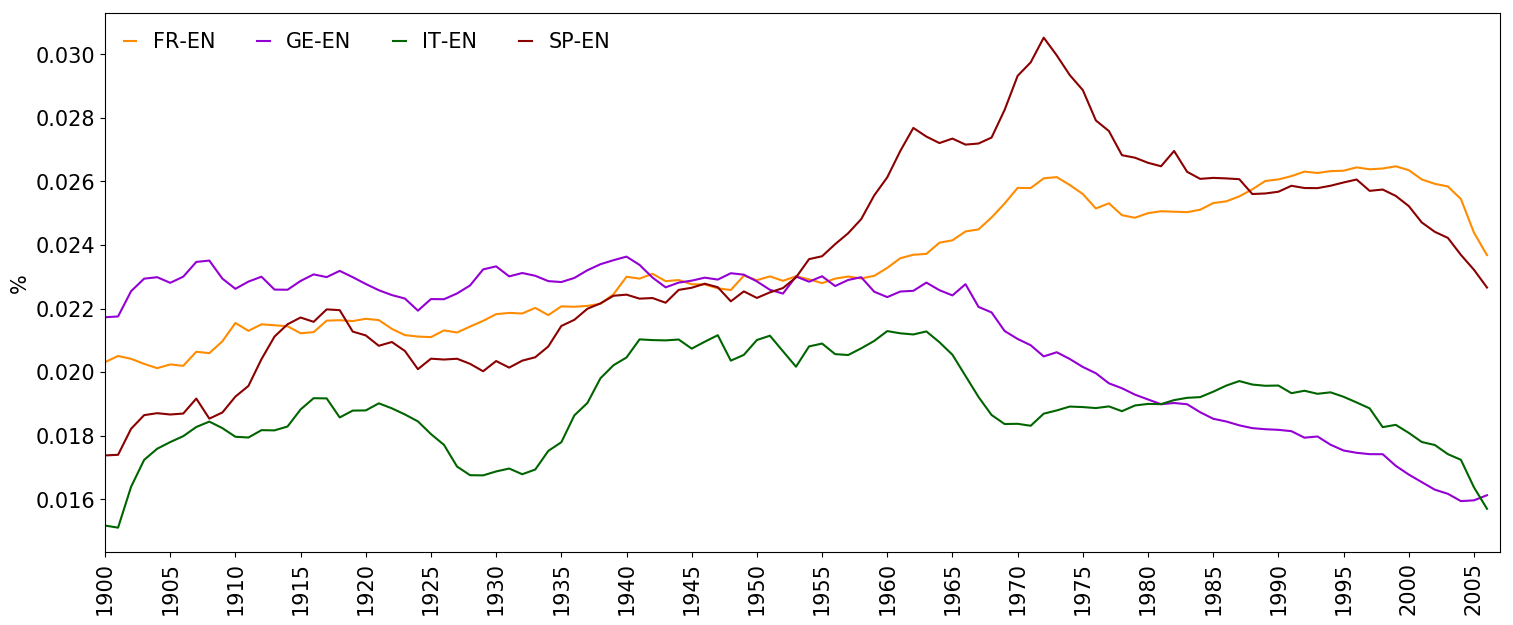
\includegraphics[scale=.36]{PF2_S2_EN.png}
	\label{fig.ST_b_EN}
	\caption{Los demás idiomas en el inglés. En los últimos 50 años, el español y el francés han sido los idiomas más utilizados. Tras la segunda guerra mundial, alemán e italiano decayeron consistente en ser lenguas de los países vencidos.}
\end{figure} 


En los últimos cincuenta años, los idiomas más utilizados  en el ingles fueron el español y el francés. Por parte del español, los préstamos continuamente utilizados son nombres de países latinoamericanos como \textit{México}, \textit{Cuba}, \textit{Chile}, \textit{Nicaragua} y \textit{Argentina};   mientras del francés, son palabras comunes en  inglés, entre ellas \textit{royals}, \textit{religion}, \textit{saint}, \textit{passage} o \textit{court}.

En alemán e italiano, su uso decayó a partir de 1960. Las palabras encontradas son referentes a la guerra y apellidos de personajes, palabras que ya se han tratado en los préstamos nuevos.




 
%Apoyado de la información de los préstamos nuevos, se puede confirmar que el inglés se ha beneficiado del crecimiento de los Estados Unidos para ser exportado a las demás lenguas y ser el idioma común para transmitir información.   

%Tras brevemente ver ambos conjuntos se infiere que el español ha logrado instaurarse en el inglés por la relevancia de estos países en las relaciones o conflictos que tuvieron en el siglo pasado y donde intervinieron países de habla inglesa, contrario  al francés que prevalece por las relaciones culturales y etimológicas que existen entre ambas lenguas.


% }}}


\subsection{Francés} % {{{

\begin{figure}%[h!]
	\centering
	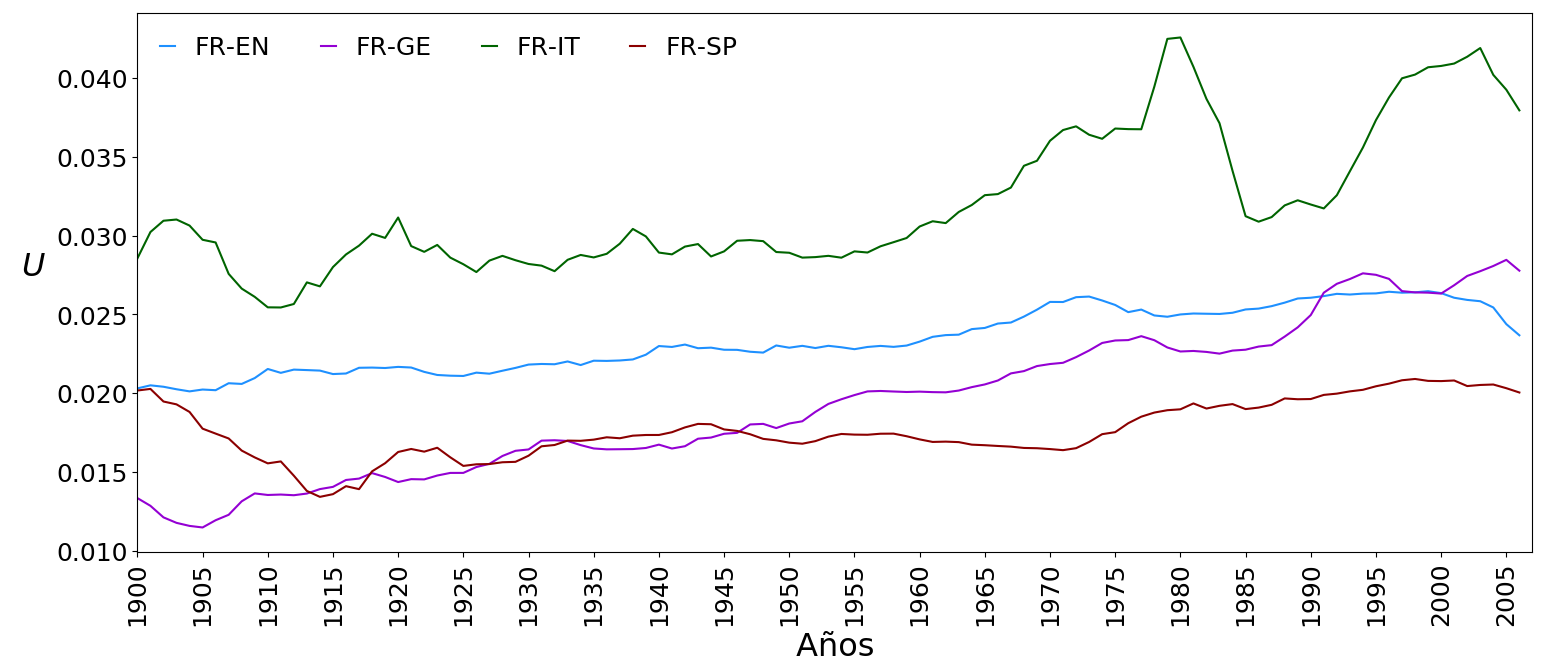
\includegraphics[scale=.36]{PF1_S2_FR.png}
	\label{fig.ST_a_FR}
	\caption{El francés en los demás idiomas. El italiano empleó más al francés durante todo el siglo XX, caracterizado por palabras comunes en la industria vitivinícola.}
\end{figure}


El italiano es el idioma que más utilizó al francés,  la industria vitivinícola, surge como un conector entre ambas lenguas al ser una actividad común en Francia e Italia, con términos como \textit{raisins}, \textit{vin}, \textit{vignoble} y \textit{recolte}.

Los préstamos hacia los demás idiomas son de carácter religioso o político, a pesar de que la búsqueda es en el siglo XX, las mayores migraciones del francés se lograron después de la revolución francesa, entre las palabras que se mantuvieron desde este acontecimiento están  \textit{saint}, \textit{eglise}, \textit{dime}, \textit{reine}, \textit{forteresse}, \textit{napoleon}, \textit{guerre}, \textit{imperiale}, \textit{bastille}, \textit{royals} o \textit{bourgeois}.  


\begin{figure}%[h!]
	\centering
	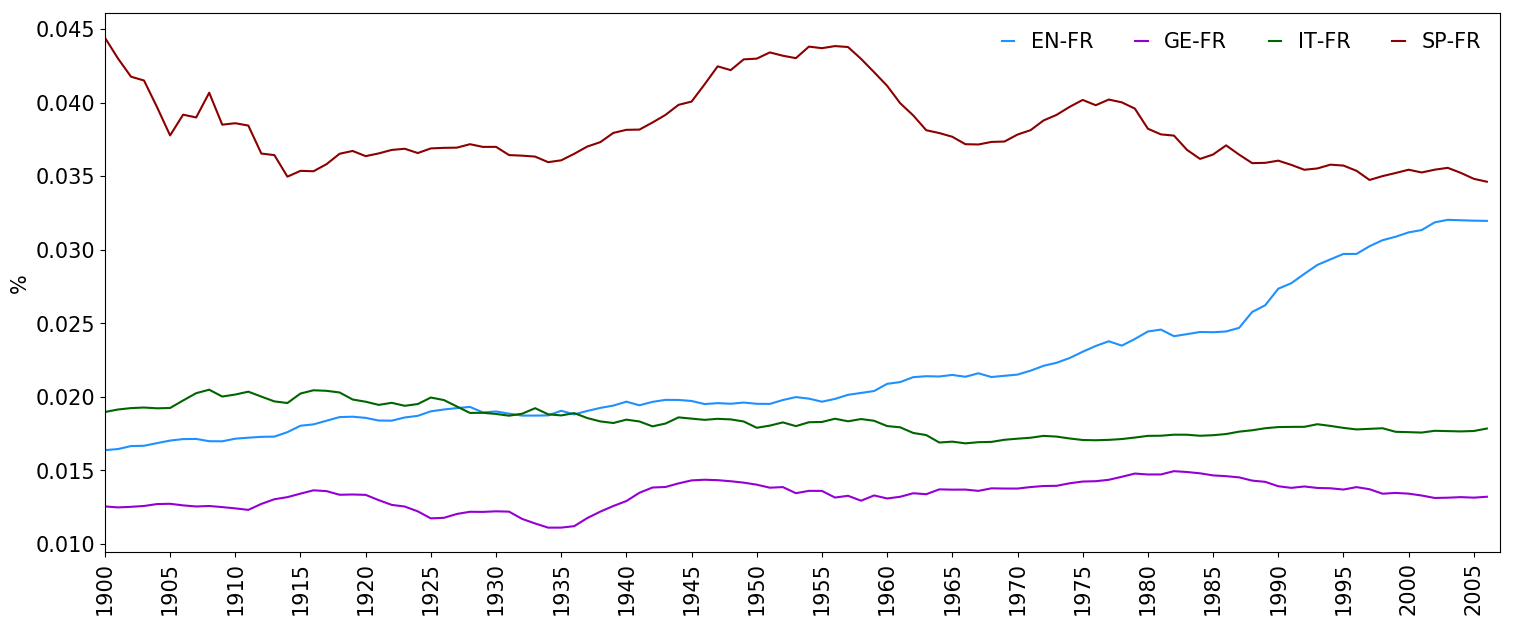
\includegraphics[scale=.36]{PF2_S2_FR.png}
	\label{fig.ST_b_FR}
	\caption{Los demás idiomas en el francés. El español ha resultado el de mayor presencia en el francés, en su mayoria son palabras con etimologías grecolatinas, comunes para ambas lenguas al provenir de la misma familia lingüística.}
\end{figure}
		
Para los prestamos usados en el francés,  español e inglés se mostraron como los idiomas con mayor presencia, siendo el español el  idioma más utilizado durante todo el siglo y el inglés el que mayor crecimiento tuvo desde 1950. La característica común de los vocablos de ambos idiomas, son palabras con etimología grecolatina,  \textit{depression}, \textit{canal}, \textit{proceso}, \textit{services}, \textit{justice} entre otras,  siendo razonable la aparición de estas palabras por tener las tres lenguas una composición grecolatina. 



\subsection{Alemán} % {{{

\begin{figure}%[h!]
	\centering
	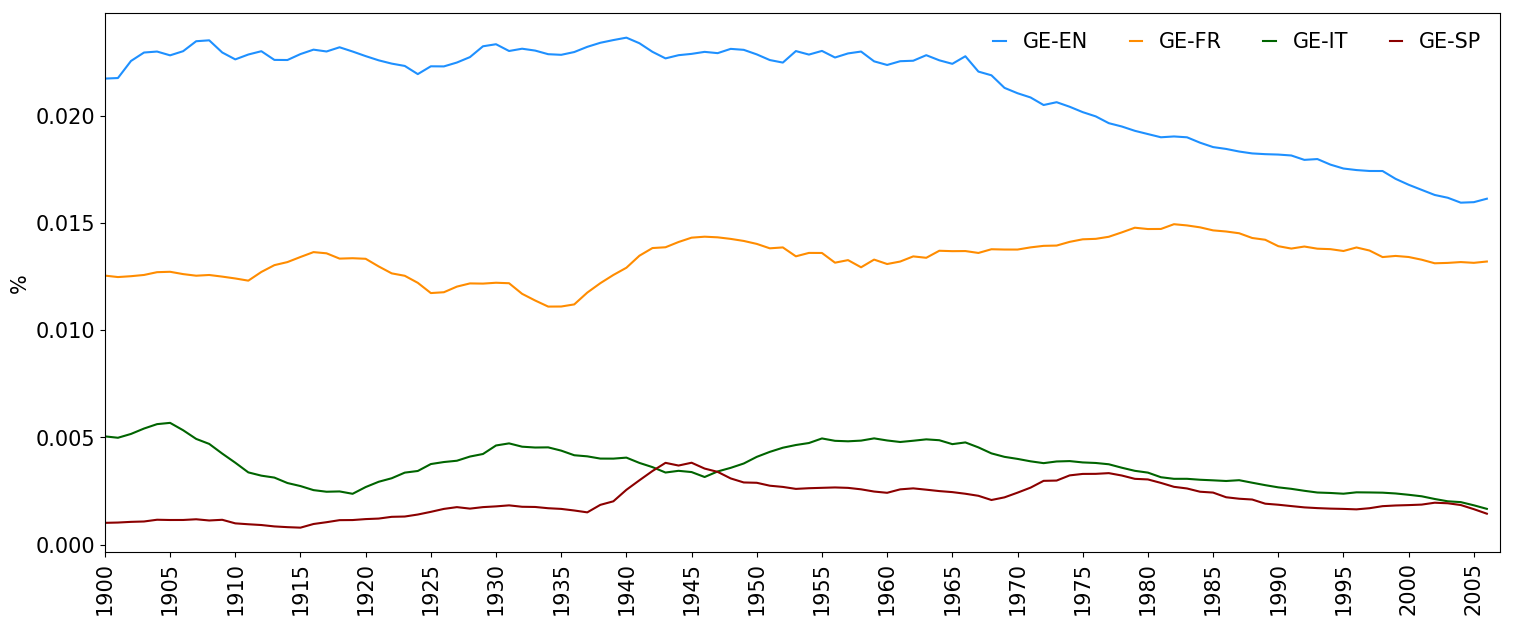
\includegraphics[scale=.36]{PF1_S2_GE.png}
	\label{fig.ST_a_GE}
	\caption{El alemán en los demás idiomas. La familiaridad de las lenguas germánicas hace posible que el inglés sea el idioma  donde los préstamos del alemán sean continuamente utilizados, siendo evidente la diferencia con las lenguas romances.}

\end{figure}

La característica principal de los términos en alemán son personajes germano-parlantes que sobresalieron en algún ámbito, \textit{Hitler}, \textit{Marx}, \textit{Einstein}, \textit{Freud}, \textit{Engels}, \textit{Heidegger}, \textit{Mozart}, \textit{Hegel} y \textit{Nietzsche}; todos ellos fueron préstamos nuevos en el slglo XX. 


\begin{figure}%[h!]
	\centering
	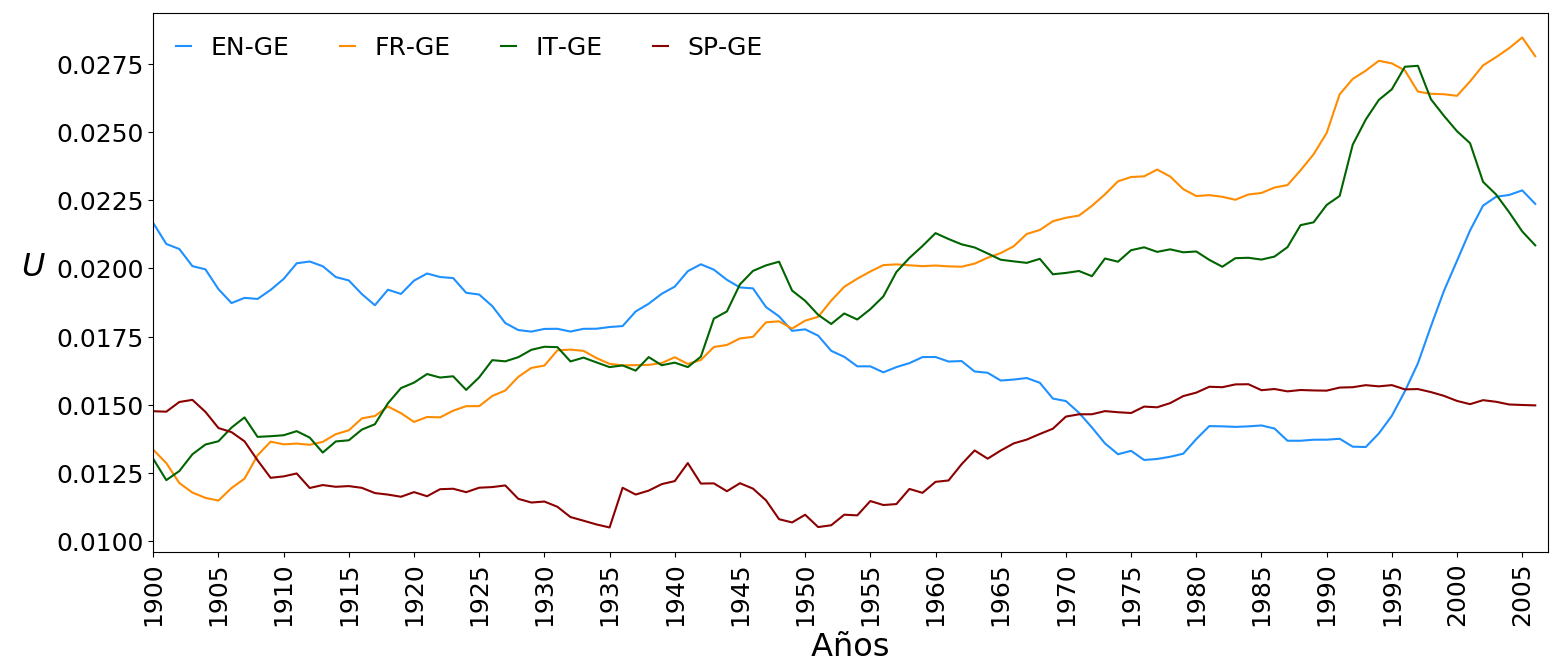
\includegraphics[scale=.36]{PF2_S2_GE.png}
	\label{fig.ST_b_GE}
	\caption{Los demás idiomas en el alemán. Cada lengua ha tenido un periodo de  crecimiento posterior a 1950 tras finalizar la segunda guerra mundial, mostrando al alemán como un idioma cambiante tras este hecho, donde los demás idiomas han impactado uy perdurado.}
\end{figure}

Como idioma receptor, el alemán adoptó palabras de diferentes campos, tecnológicos y de desarrollo por parte del inglés,  religiosos  por el francés, bélicos del italiano y médicos por el español. La mayoria de los acumulados también fueron prestamos nuevos del siglo XX. 

Cada idioma presentó un periodo de crecimiento posterior a 1950; desde el contexto histórico, al ser vencida Alemania en la segunda guerra mundial, el idioma tuvo que adaptarse a las tendencias donde los demás destacaban. 



% }}}


\subsection{Italiano} % {{{

\begin{figure}%[h!]
	\centering
	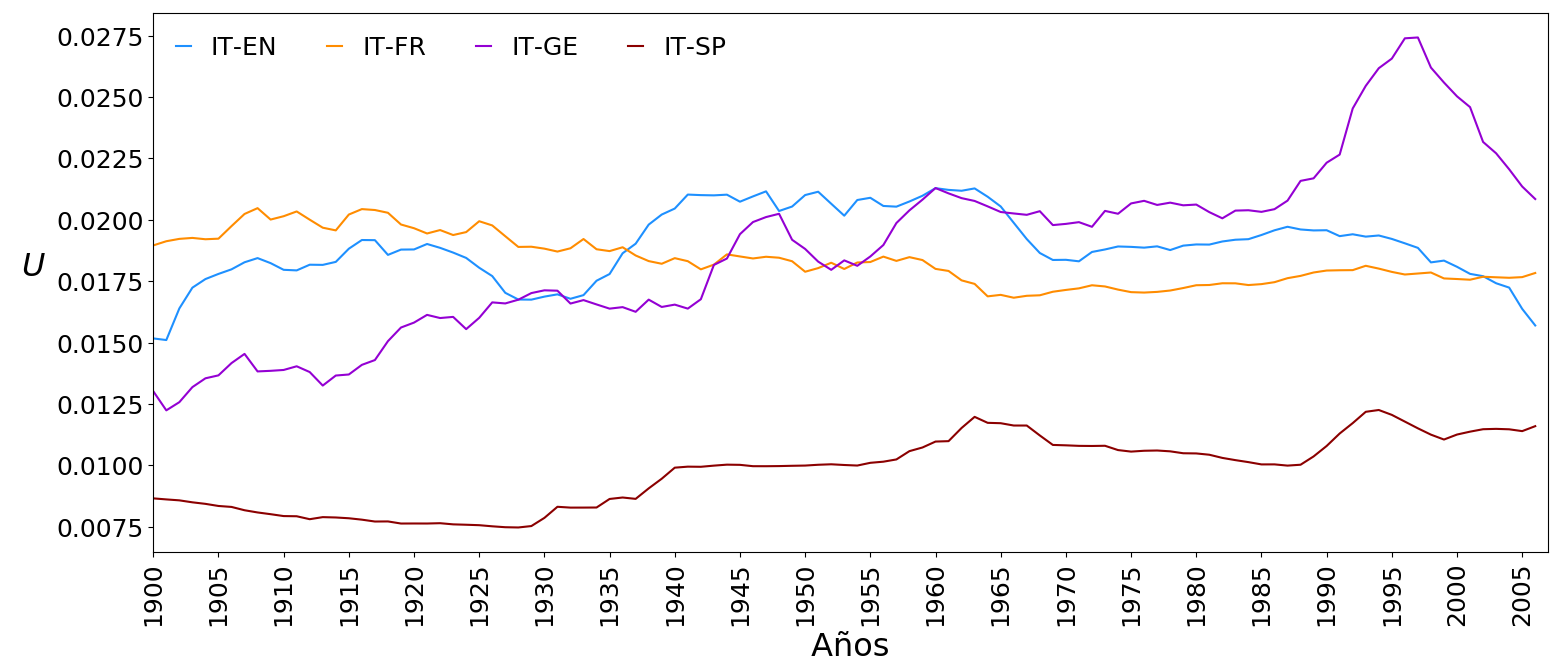
\includegraphics[scale=.36]{PF1_S2_IT.png}
	\label{fig.ST_a_IT}
	\caption{El italiano en los demás idiomas. A pesar de ser fonéticamente similares y ser tambien una lengua romance,  el español persiste en ser el idioma con menor uso de italiano.}
\end{figure}
		
		
El uso del italiano, una única palabra apareció constantemente en los demás idiomas, \textit{mussolini}, siendo el personaje más relevante en el siglo pasado, cuya lengua es el italiano.  

Salvo por Mussolini, los demás prestamos italianos no se lograron asociar a un único campo, sin embargo esto muestra la diversidad de temas en los cuales el italiano fue relevante, como la política \textit{sociale}, \textit{liberale}; la religión \textit{santo}, \textit{suora}, \textit{cattedrale}; y la guerra \textit{battaglia}, \textit{regime}.


\begin{figure}%[h!]
	\centering
	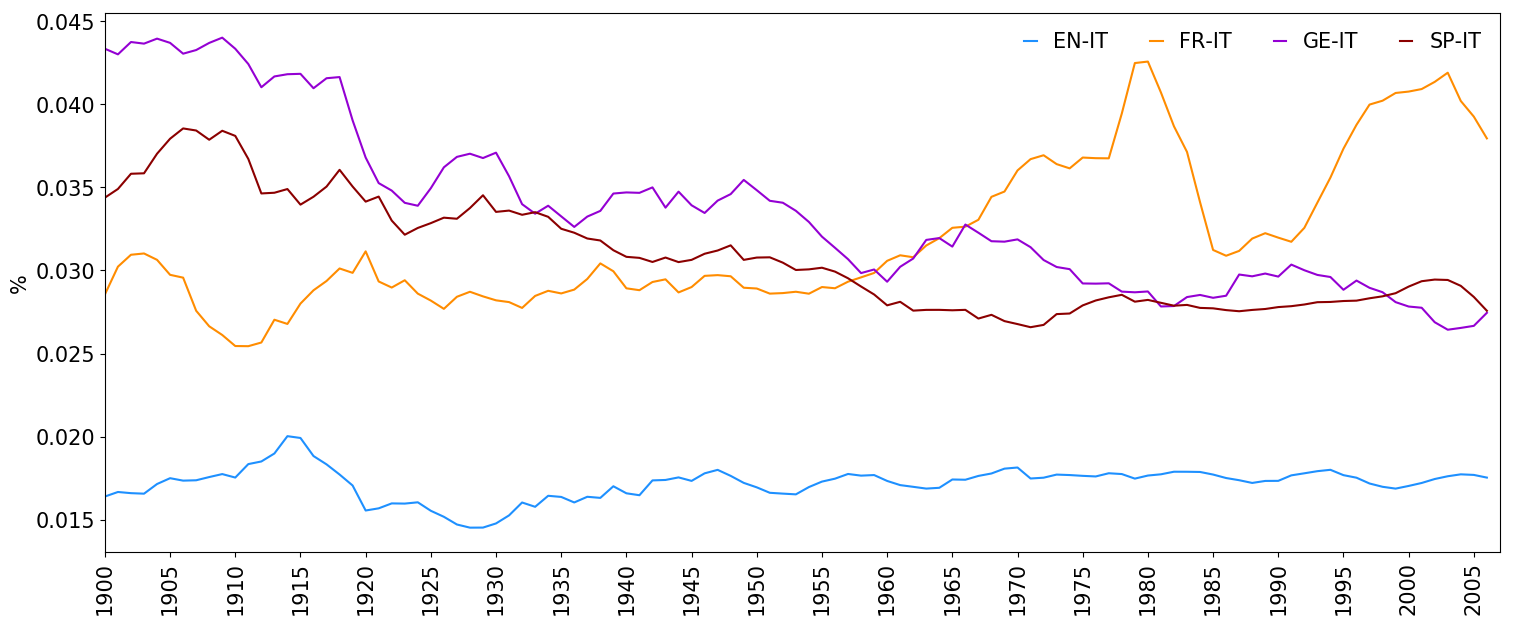
\includegraphics[scale=.36]{PF2_S2_IT.png}
	\label{fig.ST_b_IT}
	\caption{Los demás idiomas en el italiano. La proximidad geográfica  entre italia con países cuya lengua es el francés y el alemán ayudó a incrementar el uso de estos en el italiano. A pesar de que el inglés se difundió como un idioma universal para la comunicación, su uso en el italiano no ha mostrado un incremento en todo el siglo XX. }
\end{figure}

El contenido de las palabras que tomó el italiano, es igualmente variado, por parte del ingles son conceptos de la tecnología, por el francés a la industria vitivinícola, con el alemán a personajes relevantes de esta lengua, y del español a nombres de países o ciudades hispanohablantes \textit{México}, \textit{Chile}, \textit{Argentina}, \textit{Montevideo} o \textit{Peru}. 

% }}}


\subsection{Español} % {{{

\begin{figure}[h!] % {{{
	\centering
	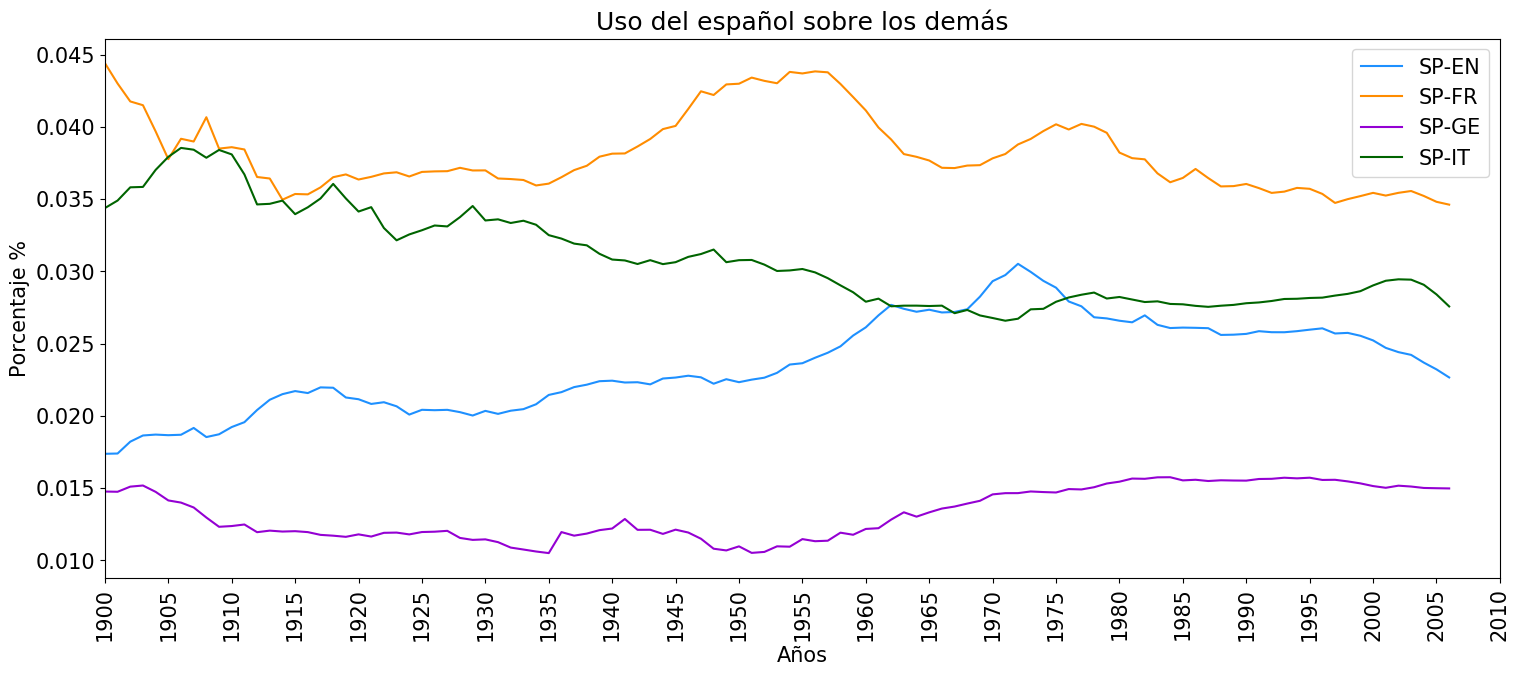
\includegraphics[scale=.36]{PF1_S2_SP.png}
	\label{fig.ST_a_SP}
	\caption{El español en los demás idiomas. Los idiomas que más emplean español son aquellos con los que comparte una relación etimológica, francés e italiano por ser lenguas romances y con el ingles al tener este idioma una base de palabras grecolatinas.  Los préstamos destacan al ser términos médicos y nombres de países y ciudades hispanohablantes.   }
\end{figure}

Entre los diferentes receptores, el francés fue el idioma que más empleo al español, seguido del italiano y dl inglés, siendo estas tres lenguas las que más relación etimológica tienen con el español.  

Entre los gráficos de la sección \ref{palabras.acumuladas.apendice}, se observo que el uso del español en los demás idiomas, es mayor que el uso de los otros en él, sin importar la combinacion que se trate.

Nuevamente,  el ámbito medico caracterizó a las palabras más empleadas con origen español, entre ellas \textit{terapia}, \textit{lepra}, \textit{tumor}, \textit{syphilis}, \textit{virus} o \textit{renal}. 

		
\begin{figure}[h!] % {{{
	\centering
	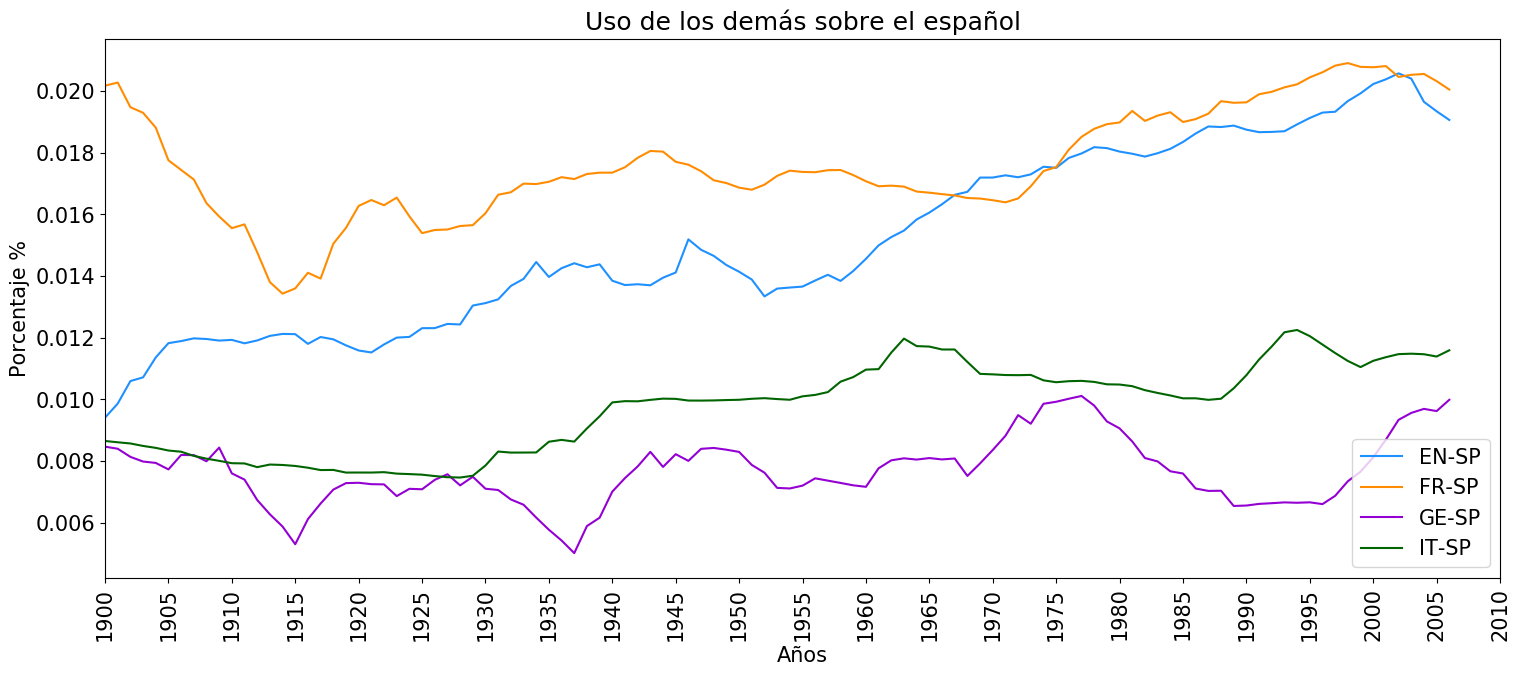
\includegraphics[scale=.36]{PF2_S2_SP.png}
	\label{fig.ST_b_SP}
	\caption{Los demás idiomas en el español.  Tanto inglés como francés han aumentado su uso  en el español, llegando a ser equiparable. El alemán ha sido el que menos ha impactado, siendo su uso casi nulo en  algunos periodos.}
\end{figure}


En las discusiones anteriores, se ha mencionado el tipo de palabras que los idiomas aportan al español, del ingles los préstamos son de carácter tecnológico y del desarrollo industrial, del alemán son apellidos de personajes destacados en un campo especifico, mientras que del francés y el italiano son tipo religioso, histórico y político. 






% }}}
% }}}
\section{Comentarios y complementos del método} % {{{


El determinar la influencia entre idiomas a través del uso, ha mostrado que el idioma que más cantidad de palabras tiene en otro no siempre es el más utilizado, radicando el mayor uso en aquel cuyos préstamos tengan menores rangos. 

Por el momento sólo es posible describir que originó las variaciones en el uso o en la cantidad de nuevas palabras, no es posible predecir como se comportaran los idiomas en el futuro. Se destaca a los eventos como una característica que  hace fluir a las palabras, alterando el uso de un idioma a tras el suceso. 

Una mejor información de como los eventos alteran a los idiomas se podría extraer si se comparará el uso con con  datos de los países de alguna habla como lo pueden ser  el crecimiento economizo, el producto interno bruto, la alfabetización, la mortalidad, las migraciones de personas, entre otros. 

%Una mejor información de como los eventos alteran a los idiomas se podría extraer si se compararán las características de los prestamos con  datos de los países de alguna habla como lo pueden ser  el crecimiento economizo, el producto interno bruto, la alfabetización, la mortalidad, las migraciones de personas, entre otros.

%En todo el siglo XX y la primer década del XXI, el inglés y el alemán han sido los idiomas más cambiantes en los papeles de origen y receptor. En cualquier combinación con otro idioma el uso ha sido alterado en alguna época. 
%El inglés al ser el que más creció en tres idiomas (francés, alemán y español), complementando los resultados del capitulo anterior, al ser el idioma que más palabras nuevas exportó.  El alemán como el receptor donde los diferentes orígenes aumentaron su usó tras la segunda guerra mundial; el uso ha sido semejante a los préstamos nuevos, ha sido el receptor que más recibió. 
%Ambos análisis se complementan,  el idioma más influyente ha aportado más palabras nuevas y aquellas que se van acumulando resultan las de mayor incremento en el uso. El idioma más influenciado recibió la mayor cantidad de palabras nuevas y el uso que han tenido los demás ha sido también el del mayor incremento. 

 




% }}}

